\section{Chemical process}\label{se:chemical_process}

\fxnote{Illustrering af fig 1,1 hvitved og dertil beskrivelse af den, for at give et overblik over kloakker og dens processer}

\subsection{Chemical reactions in a sewer}\label{subse:chemical_reactions_in_a_sewer}
A wastewater treatment plant does not only receive what is discharged into the sewer from the industry and households but also the chemical and microbial reactions that occurs in a sewer. These reaction occurs as redox reactions between the different compounds. Redox reaction is the transfer of electrons between two compounds at a atomic or molecular scale. By transferring electrons from one compound to another new compounds will rise, such as hydrogen sulfide which is know for it malodorous smell of rotten eggs. 


These redox reactions are determine to a great extend by the design of the sewer where different conditions such as aerobic, anaerobic and anoxic exist, where the last only occurs if nitrate is artificially added to the wastewater.


%The conditions are aerobic, anoxic or anaerobic. Normally aerobic and anaerobic conditions are      %These processes can affect other parts of the system e.g. some reactions may lead to malodorous substances that will reach the urban atmosphere. 



\begin{figure}[H]
\centering
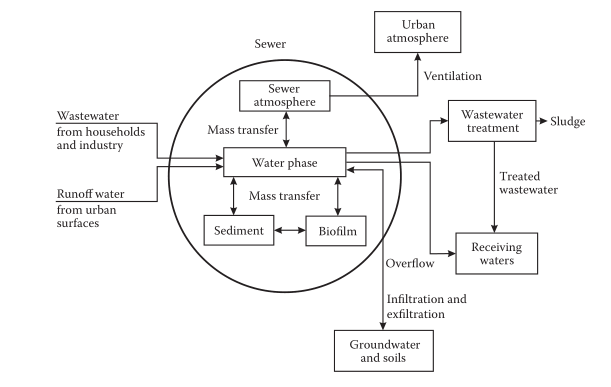
\includegraphics[width=1\textwidth]{report/introduction/pictures/sewer_overview_of_the_different_parts.png}
\caption{Illustrates how the wastewater flows from the industry and households to the treatment plant. \fxnote{Ny tegning}}
\label{fig:sewer_overview_of_the_different_parts}
\end{figure}


\subsection{Wastewater treatment plant}\label{subse:Wastewater treatment plant}

